\subsubsection{Fabric interface}
\label{sec:wrpc_fabric}

The Fabric interface is used for sending and receiving Ethernet frames. It consists 
of two pipelined Wishbone interfaces operating independently: 

\begin{itemize}
  \item \emph{WRF Source}: pipelined Wishbone Master, passes all the Ethernet frames
    received from a physical link to WRF Sink interface implemented in a
    user-defined module.
  \item \emph{WRF Sink}: pipelined Wishbone Slave, receives Ethernet frames from
    the WRF Source implemented in the user-defined module, and sends them to a
    physical link.
\end{itemize}

{\bf Address bus} can have one of the following values:

\begin{center}
\begin{tabular}{|c|l|}
  \hline {\bf decimal value} & {\bf meaning of data word on data bus}\\
  \hline
  \emph{0} & regular data (packet header and payload)\\
  \emph{1} & OOB (Out-of-band) data\\
  \emph{2} & status word\\
  \emph{3} & currently not used\\
  \hline
\end{tabular}
\end{center}

{\bf Status word} (sent when the value of address bus is \emph{2}) contains
various information about Ethernet frame's structure and type:
%\begin{figure}[ht]
  \begin{center}
    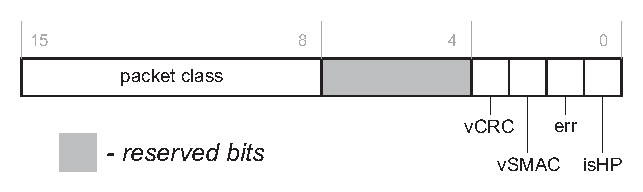
\includegraphics[width=.6\textwidth]{fig/status.pdf}
    %\caption{Status word format}
  \end{center}
%\end{figure}

\begin{itemize}
  \item[] \emph{isHP} - if \emph{1}, the frame is high priority
  \item[] \emph{err} - if \emph{1}, the frame contains an error
  \item[] \emph{vSMAC} - the frame contains a source MAC address (otherwise
    it will be assigned from WRPC configuration)
  \item[] \emph{vCRC} - the frame contains a valid CRC checksum
  \item[] \emph{packet class} - the packet class assigned by the classifier
    inside WRPC MAC module
\end{itemize}

OOB data is used for passing the timestamp-related information for the incoming and 
outgoing Ethernet frames. Each frame received from a physical link is
timestamped inside the WRPC and this value is passed as Rx OOB
data. On the other hand, for each transmitted frame the Tx timestamp can be read
from the Tx Timestamping Interface (section \ref{sec:txts}) together with a unique
frame number assigned in Tx OOB. Therefore, the format of OOB differs between Rx
and Tx frames.\\

{\bf Tx OOB format}:

%\begin{figure}[ht]
  \begin{center}
    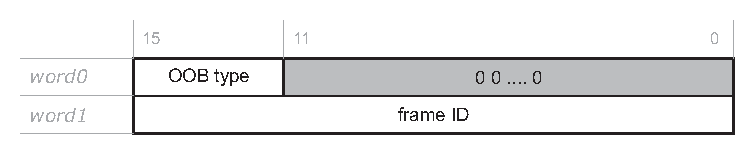
\includegraphics[width=.7\textwidth]{fig/oob_tx.pdf}
    %\caption{Tx OOB data format}
    %\label{fig:fabric_adv:tx_oob}
  \end{center}
%\end{figure}

\begin{itemize}
  \item[] \emph{OOB type}: "0001" means Tx OOB
  \item[] \emph{frame ID}: ID of the frame being sent. It is later output
    through the \emph{Tx Timestamping interface} to associate Tx timestamp with
    appropriate frame. Frame ID = 0 is reserved for PTP packets inside WRPC
    and cannot be used by user-defined modules.
\end{itemize}

{\bf Rx OOB format}:
%\begin{figure}[ht]
  \begin{center}
    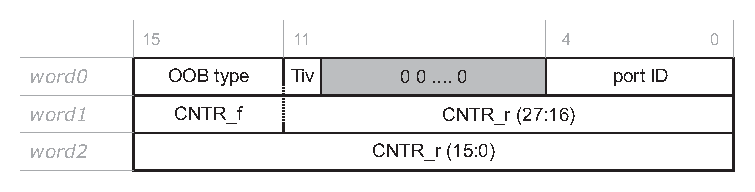
\includegraphics[width=.7\textwidth]{fig/oob_rx.pdf}
    %\caption{Rx OOB data format}
    %\label{fig:fabric_adv:rx_oob}
  \end{center}
%\end{figure}

\begin{itemize}
  \item[] \emph{OOB type}: "0000" means Rx OOB
  \item[] \emph{Tiv}: timestamp invalid. When this bit is set to '1', the PPS
    generator inside WRPC is being adjusted which means the Rx timestamp is not
    reliable.
  \item[] \emph{port ID}: the ID of a physical port on which the packet was
    received. In case of WRPC, this field is always 0, because there is only one
    physical port available.
  \item[] \emph{CNTR\_f}: least significant bits of the Rx timestamp generated on
    the falling edge of the reference clock.
  \item[] \emph{CNTR\_r}: Rx timestamp generated on the rising edge of the reference
    clock.
\end{itemize}

\begin{figure}
  \begin{center}
    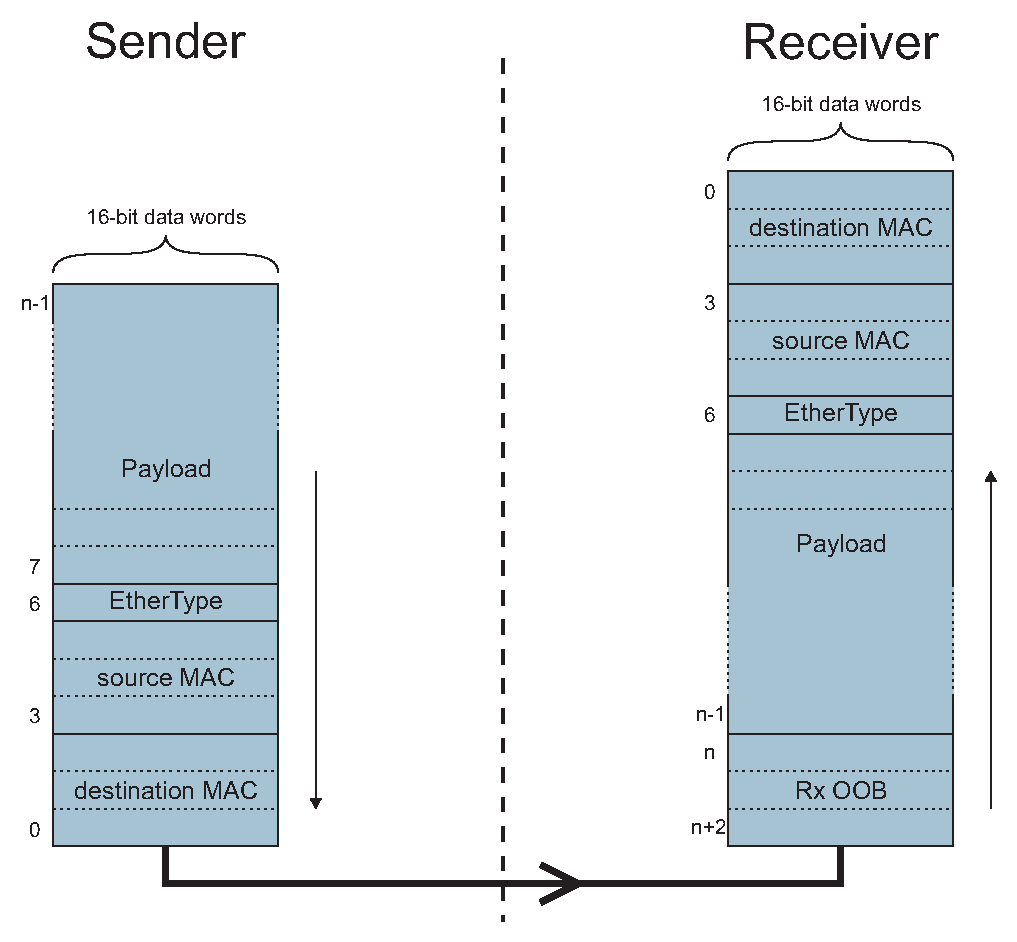
\includegraphics[width=.6\textwidth]{fig/basic_wrf_data.pdf}
    \caption{Data words that make the Ethernet frame}
    \label{fig:fabric:simple_data}
  \end{center}
\end{figure}

Figure \ref{fig:fabric:simple_data} presents data words fed to the WRF
data bus by the sender and the information got at the receiving side. Please
note that the CRC checksum is calculated and inserted automatically inside the
WRPC and user-defined module doesn't care about it. The Ethernet frame received
from the WR Fabric interface may contain additional OOB data suffixed. It has to
be received (acknowledged) by the user-defined module, but can be simply discarded.

\newparagraph{Examples}
Figure \ref{fig:fabric:simple_tx} shows a very simple WR Fabric cycle. The WRF
Source of user-defined module sends there an Ethernet frame containing even
number of bytes.

\begin{figure}
  \begin{center}
    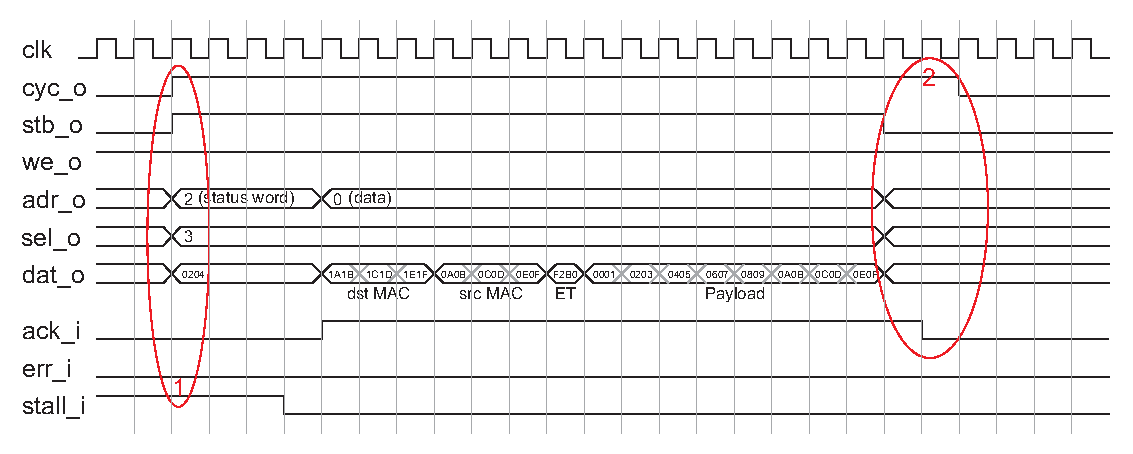
\includegraphics[width=\textwidth]{fig/basic_wrf_cycle_simple.pdf}
    \caption{Simple WR Fabric cycle - user-defined module sending packet}
    \label{fig:fabric:simple_tx}
  \end{center}
\end{figure}

\begin{enumerate}
  \item The WRF Source in user-defined module starts the cycle by asserting
    \emph{cyc\_o}, \emph{stb\_o} and putting a status word to the data bus.
    However, since WRF Sink set \emph{stall} signal to active state, Source has
    to wait until Sink is ready to receive data.
  \item After the last word is transmitted, the WRF Source sets \emph{stb\_o} back
    to \emph{0}, but waits until Sink acknowledges all the words transmitted in
    the cycle (\emph{ack\_i} line). The cycle ends when \emph{cyc\_o} goes back
    to the low state.
\end{enumerate}

Figure \ref{fig:fabric:sel} shows again a very simple WR Fabric cycle where
user-defined WRF Source sends an Ethernet frame to the WRPC. This time though,
the frame contains odd number of bytes, therefore the \emph{sel} line is used to
signal this fact to WRF Sink inside the WRPC (1).

\begin{figure}
  \begin{center}
    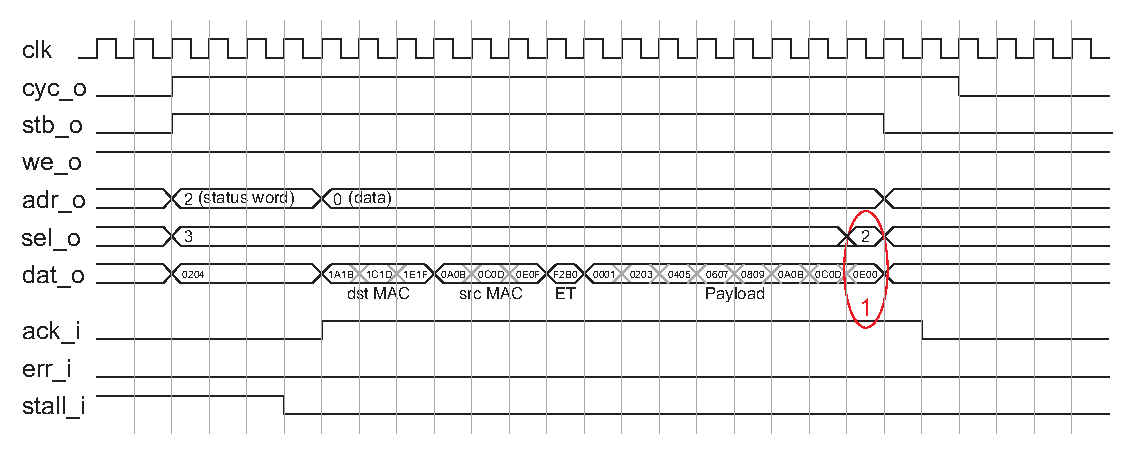
\includegraphics[width=\textwidth]{fig/basic_wrf_cycle_sel.pdf}
    \caption{Simple WR Fabric cycle - user-defined module sending packet(odd
    number of bytes in the payload)}
    \label{fig:fabric:sel}
  \end{center}
\end{figure}

Figure \ref{fig:fabric:cyc} presents more complicated Fabric cycle where an
Ethernet frame is received from WRF Source in the WRPC (output signals in the
diagram are driven by WRF Source on the WRPC side): 

\begin{figure}
  \begin{center}
    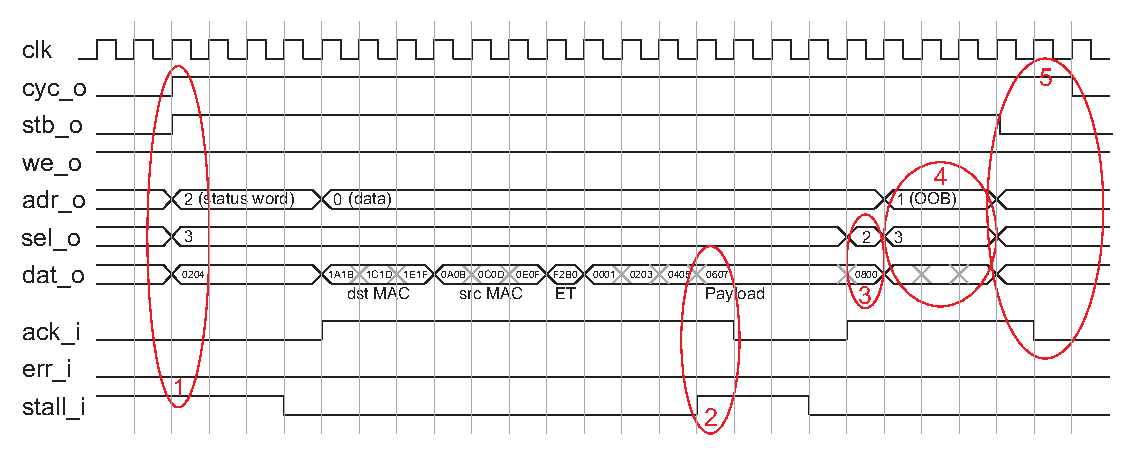
\includegraphics[width=\textwidth]{fig/basic_wrf_cycle.pdf}
    \caption{WR Fabric cycle}
    \label{fig:fabric:cyc}
  \end{center}
\end{figure}
\begin{enumerate}
  \item The WRF Source starts the cycle by asserting \emph{cyc\_o}, \emph{stb\_o}
    and putting a status word to the data bus. However, since WRF Sink set 
    \emph{stall} signal to active state, Source has to wait until Sink is ready
    to receive data.
  \item While the payload of the Ethernet frame is being transmitted, Sink
    stalls the cycle. The WRF Source pauses the transmission until Sink becomes
    ready to process the rest of the data. During that time \emph{stb\_o} has to
    remain in a high state.
  \item The Ethernet frame contains an odd number of bytes, so only half of last
    word of payload carries a valid data. \emph{Sel\_o} is used to signal this
    fact to WRF Sink.
  \item After the whole payload is transmitted, Source may additionally sent Rx
    OOB data. It contains some internal WRPC data that should be acknowledged
    by Sink, but discarded in the user's module.
  \item After the last word is transmitted, the WRF Source sets \emph{stb\_o} back
    to \emph{0}, but waits until Sink acknowledges all the words transmitted in
    the cycle (\emph{ack\_i} line). The cycle ends when \emph{cyc\_o} goes back
    to the low state.
\end{enumerate}

WRF Sink can use the \emph{stall} line to pause the frame transmission if it cannot
process the flow of data coming from WRF Source. However, if some more serious
problem appears on the receiving side, the \emph{err} line can be used to
immediately break the cycle. This situation is presented in figure
\ref{fig:fabric:cycerr}:

\begin{figure}
  \begin{center}
    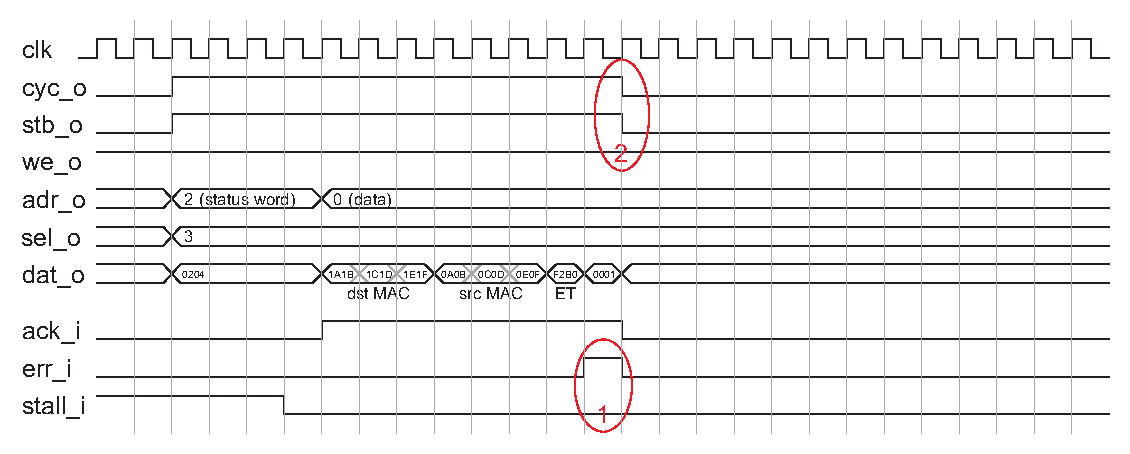
\includegraphics[width=\textwidth]{fig/basic_wrf_cycle_err.pdf}
    \caption{WR Fabric cycle interrupted with an error line}
    \label{fig:fabric:cycerr}
  \end{center}
\end{figure}

\begin{enumerate}
  \item WRF Sink wants to break a bus cycle, so it drives \emph{err\_i} high.
  \item WRF Source breaks the cycle immediately after receiving an error indicator
    from the WRF Sink.
\end{enumerate}

\newparagraph{SystemVerilog model}
The SystemVerilog simulation model of the WR Fabric interface (both WRF Source and 
WRF Sink) can be found in the \emph{wr-cores} git repository
(git://ohwr.org/hdl-core-lib/wr-cores.git) and consists of the files:
\begin{itemize}
  \item \emph{sim/if\_wb\_master.svh}
  \item \emph{sim/if\_wb\_slave.svh}
  \item \emph{sim/wb\_packet\_source.svh}
  \item \emph{sim/wb\_packet\_sink.svh}
\end{itemize}

The testbench example using the simulation model of WR Fabric interface can
be found in the zip archive attached to this documentation.

